\documentclass[acmsmall,screen]{acmart}
\usepackage{booktabs}
\usepackage{multirow}
\usepackage{makecell}
\usepackage{tikz}
\usetikzlibrary{arrows.meta,positioning,fit,calc,backgrounds}
\usepackage{algorithm}
\usepackage[noend]{algpseudocode}

\setcopyright{none}
\acmJournal{TECS}
\acmYear{2026}
\settopmatter{printacmref=false}
\renewcommand{\shortauthors}{}
\authorsaddresses{}
\renewcommand\footnotetextcopyrightpermission[1]{}
\AtBeginDocument{
  \fancypagestyle{standardpagestyle}{\fancyhf{}\fancyfoot[C]{\thepage}}
  \fancypagestyle{firstpagestyle}{\fancyhf{}}
}

\newcommand{\pol}[1]{\texttt{#1}}
\newcommand{\Wu}{$\mathcal{W}_u$}
\newcommand{\Wl}{$\mathcal{W}$}

\begin{document}

\title{Deadline Miss Early Detection for DAG Tasks with Cross-Frame State and Window Guarantees Under Intervention}

\author{Kritik Kholia, Mohit Kumar, Ayush Kumar Pal, and Dr. Swagatika Sahoo}

\begin{abstract}
Autonomous systems process sensor data through directed acyclic graphs (DAGs) of tasks, and each task chain must finish before its deadline. When a miss can be predicted early, the system can reduce the work for that frame or switch to a lighter fallback. Existing early-warning methods estimate the chance that the remaining tasks will finish on time, using each task's execution-time distribution. We show that a score based only on the current frame's elapsed time is the same for every frame at release, just when the system can most cheaply reduce the work. On embedded boards, the missing information is contention from other software, which can persist across frames. We add a state that tracks this cross-frame contention to probabilistic laxity, then place a score-independent guarantee layer above the predictor. This layer limits the long-run rate of unwarned deadline misses and the number of such misses in every window of $K$ frames, while forcing as few warnings as possible. With a lighter fallback mode, it also gives an exact bound on all late frames in each window and shows how that bound changes when the fallback is late. These guarantees continue to hold when the system acts on warnings. We also identify and fix intervention latch-up: a monitor can keep issuing warnings if its actions hide the evidence that contention has ended. Pre-registered tests on two embedded boards with a live ROS~2 LiDAR pipeline, an exhaustive theorem check and a replay of 48,000 logged release decisions confirmed the guarantees. A pre-registered replication on seven new seeds and a fallback stress test confirmed them again; across all ten UNO~Q seeds, none of 2{,}544 level-2 frames was late. The results also limit what we can claim. The predictor did not rank frames better than logistic regression. The replication did not show that the monitor reliably reduces misses at light load. On the Raspberry Pi~5 at a 6\,ms deadline, the fallback itself was sometimes late, so only the exact form of the window bound applies.
\end{abstract}

\begin{CCSXML}
<ccs2012><concept><concept_id>10010520.10010570</concept_id><concept_desc>Computer systems organization~Real-time systems</concept_desc>
<concept_significance>500</concept_significance></concept></ccs2012>
\end{CCSXML}
\ccsdesc[500]{Computer systems organization~Real-time systems}
\keywords{Deadline miss early detection, DAG, probabilistic execution time, weakly-hard constraint, adaptive conformal inference,
ROS~2, runtime monitoring}

\maketitle
\fancypagestyle{standardpagestyle}{\fancyhf{}\renewcommand{\headrulewidth}{0pt}\fancyfoot[C]{\thepage}}
\pagestyle{standardpagestyle}

% =====================================================================================================================================
\section{Introduction}\label{sec:intro}

Autonomous vehicles and mobile robots process sensor data through perception, localization and planning tasks. Each chain must finish before an end-to-end deadline. Platforms such as Autoware~\cite{kato2018autoware} organize these tasks as directed acyclic graphs (DAGs) in the Robot Operating System 2 (ROS~2)~\cite{macenski2022ros2}. On embedded multicore boards, a worst-case execution-time (WCET) analysis for the full ROS~2 graph is rarely available. Other software shares the processors and memory, so deadline misses happen in practice. A system can respond early by processing fewer points, skipping a refinement step or switching to a cheaper estimator, if it can detect the risk in time.

Azumi and colleagues have studied early detection of deadline misses in DAG tasks. Yano and Azumi~\cite{yano2023access} assigned time limits to each job based on the end-to-end deadline and WCETs, then checked each job's start time against its limit. Toba and Azumi~\cite{toba2024} replaced WCETs with probabilistic execution times and introduced probabilistic laxity, or plaxity. Toba, Baruah and Azumi~\cite{toba2026} later added probability thresholds that rise as the remaining workload shrinks. Their work provides the plaxity baseline for this paper. We ask a different question: how can a monitor use information that carries across frames and keep its guarantees after warnings trigger actions?

This work addresses two problems that arise when a detector's warnings trigger action. First, plaxity is \emph{blind at release}. It depends only on elapsed time within the current frame, and that time is zero for every frame at release. So all frames get the same score at the point when reducing a frame's workload is cheapest. This is true for any execution-time distribution and threshold (Theorem~\ref{thm:blind}). On embedded boards, contention from other software is a main cause of slow frames. It affects all nodes in a frame and can continue across frames. A method can use this information before a frame starts only if it carries state across frames. Second, \emph{detectors are not designed for intervention}. When the system degrades frames that receive warnings, it must meet three requirements:
\begin{itemize}
\item the detector's data become shaped by its own actions, and any guarantee it offers must survive this;
\item a downstream controller needs a bound on every short window of frames, not only on a long-run average;
\item a warned frame is useful only if the degraded mode actually finishes in time.
\end{itemize}

We propose a two-layer method. The \emph{prediction layer} uses the plaxity measure from Toba et al.~\cite{toba2024,toba2026}, together with a contention state carried across frames. It updates this state using completed frames and nodes that have finished in the current frame. The \emph{guarantee layer} works independently of the predictor. An adaptive threshold limits the long-run rate of unwarned misses. A counting rule limits unwarned misses in every window of $K$ frames; with a lighter fallback, it can instead limit all late frames. The predictor affects how many false alarms the method needs, but it does not affect whether the guarantees hold.

The paper makes these contributions:
\begin{itemize}
\item We prove that any early-detection score based only on elapsed time cannot distinguish frames at release, regardless of the execution-time distributions or thresholds. We then add cross-frame state to provide information before a frame begins (Sections~\ref{sec:blind} and~\ref{sec:kp}).
\item We build a predictor-independent guarantee layer: a long-run bound on unwarned misses; a lag-correct $(m,K)$ window bound with a proof that it forces the fewest possible warnings; and a bound on all late frames that accounts for late level-2 fallback frames (Sections~\ref{sec:aci}--\ref{sec:all}).
\item We identify intervention latch-up and add a state update that accounts for the operating mode. We also show why each monitor component is needed and compare the combined guarantees with bounded-miss scheduling, $(m,k)$-firm scheduling, adaptive conformal inference and weakly-hard monitoring (Sections~\ref{sec:latch} and~\ref{sec:position}).
\item We evaluate the method in pre-registered experiments on two embedded boards with a live ROS~2 pipeline. We also check the theorems exhaustively, replay the implementation decisions, and report failed tests and unsupported assumptions as well as successful results (Section~\ref{sec:eval}).
\end{itemize}

\paragraph{Scope of the claims} We do not claim that our predictor is more accurate: logistic regression using the same features ranks frames just as well (Section~\ref{sec:eval-open}). Nor do we claim that the fallback is always on time. It was late on one board at one deadline, so only the exact form of the window bound applies in that setting (Section~\ref{sec:eval-fb}). Table~\ref{tab:claims} lists each claim, its premise and its status.

Section~\ref{sec:model} describes the system. Section~\ref{sec:problem} explains the problem, the monitor requirements and how this work relates to existing methods. Section~\ref{sec:method} presents our method, and Section~\ref{sec:eval} reports the results. Section~\ref{sec:related} reviews related work. Section~\ref{sec:concl} concludes and outlines future work.

% =====================================================================================================================================
\section{System Model}\label{sec:model}

This section describes the workload, its execution times and contention, and the actions available to the monitor. Table~\ref{tab:notation} lists the notation used below.

\begin{table}[t]
\caption{Notations}
\label{tab:notation}
\footnotesize
\begin{tabular}{@{}ll@{}}
\toprule
Symbol & Description \\
\midrule
$G=(V,E)$ & DAG with nodes $V=\{\tau_1,\dots,\tau_n\}$ and edges $E$ \\
$t$ & Frame (job of the DAG) index; frame $t$ is released at time $tP$ \\
$P$, $D$ & Period and relative end-to-end deadline \\
$C_t$ & End-to-end response time of frame $t$; frame $t$ is \emph{late} if $C_t>D$ or it never finishes \\
$k$, $E_{t,k}$ & Checkpoint index ($k=0$: release) and elapsed time of frame $t$ at checkpoint $k$ \\
$\pi_k(e)$ & Plaxity: probability that the remaining nodes finish within $D-e$ \\
$z_t$ & Cross-frame contention state (log scale) \\
$s_{t,k}$ & Miss score of frame $t$ at checkpoint $k$ \\
$\theta_t$, $\alpha$, $\gamma$ & Adaptive alarm threshold, target rate, step \\
$L$ & Feedback lag: the outcome of frame $t$ is known by the release of frame $t+L$ \\
$(m,K)$ & Window budget: at most $m$ counted frames in any $K$ consecutive frames \\
$e_t$ & 1 if frame $t$ is an unwarned deadline miss, else 0 \\
$c_t$, $c^u_t$ & Window counters of rules \Wl{} and \Wu{} at the release of frame $t$ \\
\bottomrule
\end{tabular}
\end{table}

\subsection{DAG-based Workload Model}

We model the application as a DAG $G=(V,E)$. Its nodes are tasks, and its edges show how data pass between tasks. A timer releases the entry node every $P$ time units. As in~\cite{yano2023access,toba2026}, the other nodes start when data arrive from their predecessors. Each entry-node release starts a \emph{frame}; the frame ends when the exit node finishes. The exit node has a deadline $D\le P$.

Our main workload is a LiDAR perception DAG that processes nuScenes scans~\cite{caesar2020nuscenes} (Fig.~\ref{fig:sys}). N1 loads and crops each scan, and N2 voxelizes it. N3 builds a ground and obstacle grid while N4 builds a height map. N5 combines their outputs into free-space sectors. The period is $P=100$\,ms. We also test a visual-odometry DAG on EuRoC frames~\cite{burri2016euroc}, with $P=200$\,ms. Each DAG runs as five \texttt{rclcpp} nodes in one ROS~2 Jazzy process using a multi-threaded executor.

\begin{figure}[t]
\centering
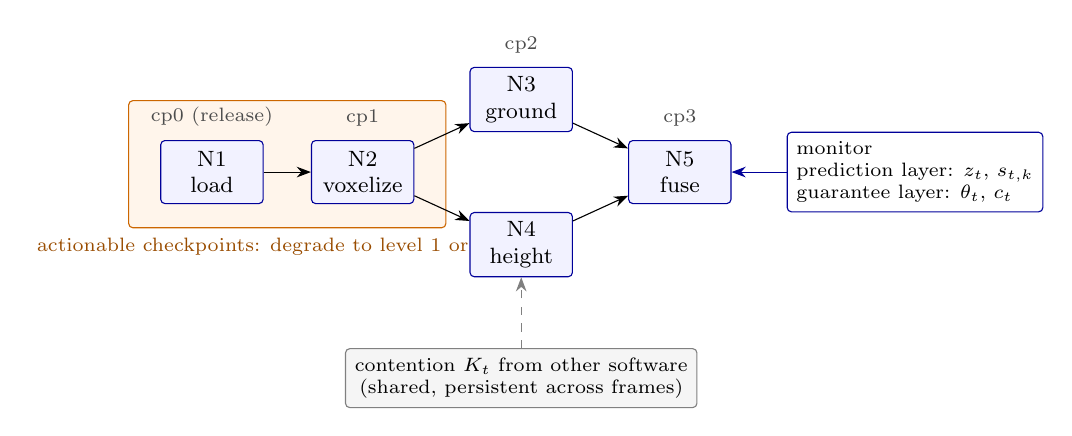
\begin{tikzpicture}[font=\footnotesize, node distance=6mm,
  nd/.style={draw=blue!60!black, fill=blue!5, rounded corners=1.5pt, minimum width=13mm, minimum height=8mm, align=center},
  cp/.style={font=\scriptsize, text=black!70}]
\node[nd] (n1) {N1\\load};
\node[nd, right=of n1] (n2) {N2\\voxelize};
\node[nd, above right=1mm and 7mm of n2] (n3) {N3\\ground};
\node[nd, below right=1mm and 7mm of n2] (n4) {N4\\height};
\node[nd, below right=1mm and 7mm of n3] (n5) {N5\\fuse};
\foreach \a/\b in {n1/n2,n2/n3,n2/n4,n3/n5,n4/n5} \draw[-{Stealth[length=1.8mm]}] (\a) -- (\b);
\node[cp, above=0.5mm of n1] {cp0 (release)};
\node[cp, above=0.5mm of n2] {cp1};
\node[cp, above=0.5mm of n3] {cp2};
\node[cp, above=0.5mm of n5] {cp3};
\begin{scope}[on background layer]
\node[draw=orange!80!black, fill=orange!8, rounded corners=1.5pt, fit=(n1)(n2), inner sep=4mm, yshift=1mm,
      label={[font=\scriptsize, text=orange!60!black]below:actionable checkpoints: degrade to level 1 or level 2}] {};
\end{scope}
\node[draw=black!50, fill=black!4, rounded corners=1.5pt, align=center, below=9mm of n4, font=\scriptsize] (cont)
      {contention $K_t$ from other software\\(shared, persistent across frames)};
\node[draw=blue!60!black, rounded corners=1.5pt, align=left, right=7mm of n5, font=\scriptsize] (mon)
      {monitor\\prediction layer: $z_t$, $s_{t,k}$\\guarantee layer: $\theta_t$, $c_t$};
\draw[-{Stealth[length=1.8mm]}, dashed, black!50] (cont) -- (n4);
\draw[-{Stealth[length=1.8mm]}, blue!60!black] (mon) -- (n5);
\end{tikzpicture}
\caption{The LiDAR DAG, its checkpoints and the monitor. Only an alarm at cp0 or cp1 leaves time to degrade the frame.}
\label{fig:sys}
\end{figure}

\subsection{Execution Time and Contention}

As in~\cite{toba2024,toba2026}, we treat each node's execution time as a random variable. We also model the main source of dependence: other software sharing the processor cores and memory. The competing workloads include Autoware reference-system processes~\cite{refsystem}, a compiler, compressors and a Python workload. The number of competing workloads, $I_t\in\{0,1,2,3\}$, changes randomly and stays at each value for an exponentially distributed time. Calibration includes $I_t\in\{0,1,2\}$. Validation adds $I_t=3$ and, in later tests, a workload type not used in calibration. Contention slows all the nodes in a frame and can persist into later frames, so execution times depend on one another within and across frames.

\subsection{Monitor, Actions and Fallback Modes}

The monitor checks each frame at four points (Fig.~\ref{fig:sys}): release (cp0), the start of N2 (cp1), the start of the fork (cp2), and the start of N5 (cp3). An alarm at cp0 or cp1 is \emph{actionable}: the system can still reduce the work. \emph{Level~1} keeps every second scan point; \emph{level~2} keeps every eighth. Both reduce the work in N2--N5. A frame is \emph{warned} if it is degraded at release or triggers an alarm at cp0 or cp1. An \emph{unwarned deadline miss} is a late frame that received no warning. The monitor learns whether frame $t$ was late when that frame finishes. Until then, the frame is \emph{running}. The feedback lag $L$ is the maximum number of later releases that can occur before the outcome is known.

% =====================================================================================================================================
\section{Problem Model}\label{sec:problem}

This section defines the problem. Section~\ref{sec:blind} explains why per-frame detection cannot distinguish frames at release. Section~\ref{sec:req} lists what a monitor must guarantee when its warnings trigger action. Section~\ref{sec:position} compares those requirements with existing methods.

\subsection{Release-Time Blindness of Per-Frame Early Detection}\label{sec:blind}

At checkpoint $k$ and elapsed time $e$, plaxity~\cite{toba2024,toba2026} is $\pi_k(e)=\Pr[R_k\le D-e]$. Here $R_k$ is the sum, under convolution, of the execution-time distributions for the unfinished nodes. The detector raises an alarm when $\pi_k(e)$ falls below threshold $th_k$, which increases near the exit node~\cite{toba2026}. After calibration, $\pi_k$ is fixed; during a run, it depends only on the current frame's elapsed time. Let $\mathcal I_{t,k}$ be the information available at checkpoint $k$ of frame $t$, and let $Y_t=\mathbf 1[C_t>D]$.

\begin{theorem}[Release-time blindness]\label{thm:blind}
Let $s_{t,k}=g_k(E_{t,k})$ for fixed functions $g_k$; this includes plaxity with any distributions, fork rule and thresholds. Then
(i) at release, $s_{t,0}=g_0(0)$ for every frame, its AUROC for $Y_t$ is exactly $1/2$, and every threshold raises an alarm on all frames
or on none; (ii) if $g_k$ is monotone, the ROC curve of $s_{t,k}$ is dominated by that of $E_{t,k}$ itself.
\end{theorem}
\begin{proof}
(i) Since $E_{t,0}=0$ for every frame, all frames get the same score. Every late/on-time pair is tied, and a threshold on a constant score alarms on either every frame or none. (ii) A strictly monotone change to a score leaves its ROC curve unchanged. A non-strictly monotone change can merge scores into ties, replacing parts of the curve with straight chords.
\end{proof}

\begin{proposition}[Information limit]\label{prop:limit}
Among $\mathcal I_{t,k}$-measurable scores, $p^\star_{t,k}=\Pr[Y_t=1\mid\mathcal I_{t,k}]$ has the highest ROC curve, and enlarging
$\mathcal I_{t,k}$ cannot lower it. If $\log C_t=S_t+\varepsilon_t$ with a state $S_t$ known at release and independent Gaussian noise
$\varepsilon_t$, the best release-time AUROC depends only on $R^2=\mathrm{Var}(S_t)/\mathrm{Var}(\log C_t)$ and on the miss rate.
\end{proposition}
\begin{proof}
The Neyman--Pearson lemma says that, at any false-positive rate, the strongest test thresholds the likelihood ratio. That ratio is a monotone function of $p^\star_{t,k}$. Also, any score based on $\mathcal I'$ is available when the monitor has the larger information set $\mathcal I$, if $\mathcal I'\subseteq\mathcal I$. In the Gaussian case, $p^\star_{t,0}$ increases monotonically with $S_t$.
\end{proof}

Theorem~\ref{thm:blind} shows that changing the execution-time distributions cannot make a per-frame detector distinguish frames at release. To detect risk at that point, a method needs information from before the frame starts. Proposition~\ref{prop:limit} describes the best a method can do with that information.

\subsection{Requirements for a Monitor That Is Acted Upon}\label{sec:req}

When no WCET analysis is available, a monitor that triggers degradation should meet six requirements:
\begin{description}
\item[R1] It warns at release, when degradation is cheapest.
\item[R2] It gives a hard $(m,K)$ bound in every window of $K$ frames, not only a long-run rate.
\item[R3] R2 still holds when outcomes become known only after a lag $L\ge1$, the normal case in a pipelined system.
\item[R4] Its guarantees remain valid when its own actions shape the data from which it learns.
\item[R5] It bounds \emph{all} late frames, not only unwarned ones, and states how the bound degrades when the fallback is late.
\item[R6] A learned predictor decides only the false-alarm price, never whether a guarantee holds.
\end{description}

\subsection{What Existing Mechanisms Provide, and What They Do Not}\label{sec:position}

Prior work provides some of the pieces used by our method. Here we explain what those methods provide, what we use, and what we add. Table~\ref{tab:compare} summarizes the comparison, following~\cite{toba2026}.

\begin{table}[t]
\caption{How the proposed method compares with related work. \checkmark: provided; $\circ$: provided only with the stated extra assumption; --: not provided or outside the work's scope.}
\label{tab:compare}
\footnotesize
\begin{tabular}{@{}lccccccc@{}}
\toprule
Work & DED$^a$ & R1 & R2 & R3 & R4 & R5 & R6 \\
\midrule
Yano and Azumi, IEEE Access 2023~\cite{yano2023access} & \checkmark & -- & -- & -- & -- & -- & -- \\
Toba and Azumi, ECRTS 2024~\cite{toba2024}; Toba et al., TECS 2026~\cite{toba2026} & \checkmark & -- & -- & -- & -- & -- & -- \\
Bernat and Cayssials, RTSS 2001 (Bi-Modal Scheduler)~\cite{bernat2001bms} & -- & -- & $\circ^b$ & $\circ^c$ & -- & $\circ^b$ & -- \\
Hamdaoui and Ramanathan, TC 1995 ($(m,k)$-firm)~\cite{hamdaoui1995} & -- & -- & $\circ^b$ & $\circ^c$ & -- & -- & -- \\
Gibbs and Cand\`es, NeurIPS 2021 (ACI)~\cite{gibbs2021} & -- & -- & -- & \checkmark & $\circ^d$ & -- & \checkmark \\
Peeck et al., DATE 2021~\cite{peeck2021} & \checkmark$^e$ & -- & $\circ^f$ & -- & -- & $\circ^g$ & -- \\
Wu et al., RV 2020~\cite{wu2020rv} & -- & -- & $\circ^h$ & -- & -- & -- & -- \\
Jiang et al., RTSS 2020 (Pythia-MCS)~\cite{jiang2020pythia} & \checkmark & $\circ^i$ & -- & -- & -- & -- & -- \\
Proposed method & \checkmark & \checkmark & \checkmark & \checkmark & \checkmark & \checkmark$^j$ & \checkmark \\
\bottomrule
\end{tabular}

\vspace{2pt}
\parbox{\textwidth}{\scriptsize
$^a$ DED: deadline miss early detection at run time.
$^b$ Given a schedulability (WCET) analysis that guarantees the switched-to mode.
$^c$ Outcomes known at each job's deadline.
$^d$ Long-run rate only; the bound is sequence-wise.
$^e$ Detection after a segment budget is overrun.
$^f$ $(m,k)$ checked on measured traces when the budgets are set; not enforced online.
$^g$ Fallback to a safety layer whose timing is assumed.
$^h$ The system is verified \emph{if} the environment satisfies the constraints; otherwise it switches to a safe mode.
$^i$ Before the overrun, from I/O behaviour, to trigger a mixed-criticality mode switch.
$^j$ Exact form without assumption; plain form only when the fallback is on time.}
\end{table}

\paragraph{Bounded-miss scheduling} The Bi-Modal Scheduler of Bernat and Cayssials~\cite{bernat2001bms} runs jobs in best-effort mode, then switches to a guaranteed panic mode before another miss would violate the weakly-hard constraint~\cite{bernat2001weakly}. $(m,k)$-firm scheduling~\cite{hamdaoui1995} raises a stream's priority as it approaches a violation. Both count misses in a window. Our counting rules use the same basic idea; we do not claim that idea as new. These schedulers rely on timing analysis to show that the guaranteed mode or prioritized job will meet its deadline. Our method differs in three ways. (i) The window bound on unwarned misses (Theorem~\ref{thm:wu}) needs no timing analysis. It warns a frame, which the monitor can always do, rather than relying on that frame to meet its deadline. (ii) Its counter handles a feedback lag $L$. Counting only known misses, as a scheduler might at each deadline, can allow $m+L-1$ misses (Proposition~\ref{prop:need}). (iii) For all late frames, Theorem~\ref{thm:all} gives an exact bound even when the fallback is late. This makes the timing assumption in bounded-miss scheduling explicit and measurable. If $L=1$, the predictor never warns, and the fallback never misses, rule \Wl{} switches modes under the same condition as the panic mode in~\cite{bernat2001bms}.

\paragraph{Adaptive conformal inference} The long-run bound in Section~\ref{sec:aci} is the one-sided adaptive conformal inference (ACI) bound of Gibbs and Cand\`es~\cite{gibbs2021}, adjusted for feedback lag. We do not claim this bound as new. ACI alone gives no window bound: Proposition~\ref{prop:need}(2) shows that even a valid ACI threshold can allow $\lfloor\theta_1/(\gamma(1-\alpha))\rfloor$ consecutive unwarned misses. It also gives no bound on late frames. Our contribution is to use ACI as one layer of an actionable monitor. Its bound still holds after intervention because it applies to each sequence and is defined only for unwarned frames.

\paragraph{Weakly-hard monitoring} Peeck, Schlatow and Ernst~\cite{peeck2021} monitor event-chain latency using segment timeouts and switch to a safety layer. They choose segment budgets from measured traces so that the $(m,k)$ requirement holds on those traces. Wu et al.~\cite{wu2020rv} verify systems against several weakly-hard constraints and switch to a safe mode when the environment violates them. These methods detect or verify a weakly-hard property. They do not enforce it online by requiring warnings or degradation, and a timeout detects a problem only after a budget is exceeded. Our method enforces $(m,K)$ by construction, with proofs that do not rely on measured traces.

\paragraph{What the proposed method adds} Our contribution is how these pieces work together:
\begin{enumerate}
\item Every guarantee follows from a counter or threshold update. The proofs need no timing model and no assumptions about the predictor, so a learned predictor can be used with a hard window guarantee.
\item Running frames are counted correctly despite feedback lag, and we prove that the rule cannot force fewer warnings.
\item The guarantees remain valid when the monitor intervenes. We also identify and fix latch-up, the practical failure caused by intervention.
\item The exact window bound on all late frames needs no timing assumption. It makes fallback timing explicit and measurable.
\item Cross-frame state can warn at release, when per-frame detection cannot distinguish frames.
\end{enumerate}
The proofs are short. The next proposition shows why each component is needed.

\begin{proposition}[Each component is necessary]\label{prop:need}
Consider the proposed method with one component removed.
\begin{enumerate}
\item Without cross-frame state, the release decision is the same for every frame (Theorem~\ref{thm:blind}).
\item With the adaptive threshold but no window rule, scores identically 0 and every frame late, the first
$\lfloor\theta_1/(\gamma(1-\alpha))\rfloor$ frames are unwarned misses, so no $(m,K)$ bound holds for $K\le\theta_1/(\gamma(1-\alpha))$
although Theorem~\ref{thm:aci} holds.
\item If the window counter ignores running frames, the worst number of unwarned misses in a window is exactly $\min(m+L-1,K)$.
\item With a window rule on unwarned misses only, every warned frame may be late, so up to $K$ late frames per window are possible
while Theorem~\ref{thm:wu} holds.
\item If the state is updated only from undegraded frames and the monitor degrades every frame after a contention burst, the state never
decreases. With a fixed threshold every later frame is degraded; with the adaptive threshold the latch ends only after the threshold has
risen above the stale score $s$, which takes $(s-\theta_t)/(\gamma\alpha)$ frames and leaves the threshold loosened.
\end{enumerate}
\end{proposition}
\begin{proof}
(1) is Theorem~\ref{thm:blind}. (2) With scores 0, frame $t$ is warned only if $\theta_t<0$, and each fed-back unwarned miss lowers
$\theta$ by $\gamma(1-\alpha)$. (3) At the release of $t$ the frames $t-L+1,\dots,t-1$ may be running and are not counted; with $m-1$
known unwarned misses in the window, $t$ is released unwarned, and an adversary makes the $L-1$ running frames and $t$ late, which gives
$m+L-1$. The upper bound follows from the argument of Theorem~\ref{thm:wu} with $L-1$ uncounted frames. (4) Nothing constrains the
latency of a warned frame. (5) The release prior is a function of undegraded outcomes only; when none arrive it is constant, and a
degraded frame is warned, so $e_t=0$ and $\theta$ rises by $\gamma\alpha$ per frame.
\end{proof}

% =====================================================================================================================================
\section{Proposed Method}\label{sec:method}

This section explains the predictor (Section~\ref{sec:kp}), the three guarantees (Sections~\ref{sec:aci}--\ref{sec:all}), the latch-up fix (Section~\ref{sec:latch}) and the complete algorithm (Section~\ref{sec:alg}).

\subsection{Cross-Frame State: Kalman Plaxity}\label{sec:kp}

Our predictor keeps plaxity's score, checkpoints and convolution~\cite{toba2024,toba2026}, and adds a state for contention. Let $z_t$ be the log-scale contention state. At the release of frame $t$, its prior mean is an exponentially weighted average of $\log(C_j/\bar C)$ across completed frames $j<t$, where $\bar C$ is the median latency during calibration. As each node $i$ finishes, its duration relative to its calibration median gives a scalar Gaussian observation of $z_t$. We estimate the remaining time as $e^{z_t}$ times the convolution of the state-normalized node durations, represented by 64 quantiles. The resulting score is $s_{t,k}=\Pr[E_{t,k}+R_k>D\mid z_t]$. We call this predictor Kalman plaxity (KP). A second version, KPF, also forms a prior from CPU and memory counters collected by a background sampler. It combines the two priors online, weighting each by its recent squared prediction error. The predictor runs inside the ROS~2 process and is implemented in C++.

\subsection{Long-Run Guarantee on Unwarned Deadline Misses}\label{sec:aci}

A frame raises an alarm at the first actionable checkpoint at which $s_{t,k}>\theta_t$. When the outcome of frame $t-L$ becomes known,
the threshold is updated as $\theta_{t+1}=\theta_t-\gamma(e_{t-L}-\alpha)$.

\begin{theorem}[Long-run bound]\label{thm:aci}
For any scores in $[0,1]$ and any sequence of response times, including sequences shaped by the monitor's own interventions,
\[\frac1T\sum_{t\le T}e_t\;\le\;\alpha+\frac{\theta_1+(L+1)\gamma}{\gamma T}+\frac LT.\]
\end{theorem}
\begin{proof}
If $\theta_t<0$, every score is above the threshold, so $e_t=0$. The threshold can therefore drop only after an unwarned miss released when $\theta\ge0$. After that, at most $L+1$ updates can lower it, each by at most $\gamma$. Thus $\theta_t\ge-(L+1)\gamma$ for every $t$. Summing the update gives $\sum_{u\le T-L}(e_u-\alpha)=(\theta_1-\theta_{T+1})/\gamma\le(\theta_1+(L+1)\gamma)/\gamma$. The final $L$ terms add at most $L$.
\end{proof}
This proof assumes neither exchangeability nor stationarity, so it applies to each sequence. The monitor defines $e_t$ only for unwarned frames, which run without modification. Its actions therefore do not change this measurement. The bound is one-sided, on the safety-relevant quantity.

\subsection{Window Guarantee on Unwarned Deadline Misses}\label{sec:wu}

\begin{definition}[Rule \Wu]
Before releasing frame $t$, let $c^u_t=\#\{j\in[t-K+1,t-1]: j$ is a known unwarned miss, or $j$ is unwarned and running$\}$. If
$c^u_t\ge m$, frame $t$ is warned at release (degraded to level~1).
\end{definition}

\begin{theorem}[$(m,K)$ on unwarned misses]\label{thm:wu}
Under rule \Wu, for every predictor, every response-time sequence and every lag, every window of $K$ consecutive frames contains at most
$m$ unwarned deadline misses.
\end{theorem}
\begin{proof}
Assume a window contains $m+1$ unwarned misses, and call the last one $f$. Because $f$ was not warned, the rule had $c^u_f<m$. But the other $m$ misses fall within $[f-K+1,f-1]$. When $f$ was released, each was either a known unwarned miss or still running and unwarned. The counter must therefore have been at least $m$, a contradiction.
\end{proof}

\begin{proposition}[Minimality]\label{prop:min}
Any causal policy that guarantees $(m,K)$ on unwarned misses for every response-time sequence must warn every frame that rule \Wu{}
forces.
\end{proposition}
\begin{proof}
If $c^u_t\ge m$, an adversary can choose outcomes consistent with what the monitor has seen so that every counted running frame and frame $t$ are late. If the monitor does not warn frame $t$, the window $[t-K+1,t]$ then has $m+1$ unwarned misses.
\end{proof}

Minimality means the monitor cannot omit any warning forced by the rule; it does not say how many warnings the rule will force. The next theorem bounds that cost using the unwarned-miss count controlled by the long-run layer. This connects the two parts of the guarantee.

\begin{theorem}[Price of the window rule]\label{thm:cost}
Over any horizon of $T$ frames, let $F$ be the number of frames forced by rule \Wu, $U$ the number of unwarned deadline misses and $N$
the number of unwarned frames. For every predictor, every response-time sequence and every lag~$L$,
\[ mF \;\le\; (K-1)\,U + (L-1)\,N. \]
\end{theorem}
\begin{proof}
Every forced frame has $c^u_t\ge m$, so $mF\le\sum_t c^u_t$. An unwarned frame $j$ can contribute to later counters only for $t\in[j+1,j+K-1]$. If $j$ is a miss, it contributes at most $K-1$ times. If it is on time, it contributes only while still running, for at most $L-1$ releases. Summing these contributions over all frames gives the bound.
\end{proof}

\begin{corollary}[Forced-warning rate]\label{cor:cost}
If the threshold of Section~\ref{sec:aci} runs together with rule \Wu, then for $L=1$
\[ \frac FT\;\le\;\frac{K-1}{m}\left(\alpha+\frac{\theta_1+2\gamma}{\gamma T}+\frac1T\right). \]
\end{corollary}
\begin{proof}
Forced frames are warned, so they cannot add to $U$. Theorem~\ref{thm:aci} therefore still bounds $U$ under the combined policy. Substituting that bound into Theorem~\ref{thm:cost} gives the result.
\end{proof}

The two layers work together. The long-run layer keeps the unwarned-miss rate near $\alpha$, which limits the fraction of frames forced by the window rule to $(K-1)\alpha/m$, regardless of the predictor or response times. If $m/(K-1)$ is much larger than $\alpha$, the window rule is inexpensive. If it is smaller, the rule may force many warnings, as seen in Section~\ref{sec:eval-disc}. For $L=1$, the bound is close to tight. Exhaustive enumeration (Section~\ref{sec:eval-verify}) found the maximum $mF/U$ to be exactly $K-m$. This occurs in blocks of $m$ consecutive unwarned misses, each forcing warnings on the next $K-m$ releases.

\subsection{Window Guarantee on All Late Frames with a Fallback}\label{sec:all}

\begin{definition}[Rule \Wl]
Before releasing frame $t$, let $c_t=\#\{j\in[t-K+1,t-1]: j$ is known late, or $j$ is running and not at level~2$\}$. If $c_t\ge m$,
frame $t$ runs at level~2. Otherwise the prediction layer and the adaptive threshold decide between normal mode and level~1.
\end{definition}

\begin{theorem}[All late frames, exact form]\label{thm:all}
Under rule \Wl, for every response-time sequence and every lag, every window $W$ of $K$ frames satisfies
\[\#\{\text{late frames in }W\}\;\le\;m+\#\{\text{late level-2 frames in }W\}.\]
\end{theorem}
\begin{proof}
It is enough to show that $W$ contains at most $m$ late frames that did not run at level~2. Suppose instead there are $m+1$, and let $f$ be the last. Since $f$ did not run at level~2, its counter had $c_f<m$. The other $m$ frames are in $[f-K+1,f-1]$. When $f$ was released, each was either known to be late or still running at a level other than~2. So $c_f\ge m$, a contradiction.
\end{proof}

Theorem~\ref{thm:all} makes no timing assumption. It only requires the monitor to count a frame as running until its outcome is known; our implementation does this (Section~\ref{sec:eval-verify}). Additional evidence can support two simpler bounds.

\begin{corollary}[Budgeted form]\label{cor:r}
If at most $r$ level-2 frames are late in any window of $K$ frames, every window contains at most $m+r$ late frames.
\end{corollary}

\begin{corollary}[Plain form]\label{cor:A}
If level-2 frames are never late (assumption A), every window of $K$ frames contains at most $m$ late frames.
\end{corollary}

Assumption A depends on the platform, deadline, contention and scheduling setup, not on the monitor. A finite test can estimate the \emph{rate} of late level-2 frames, but it cannot prove that no such frame will ever be late. A deterministic plain bound needs a WCET limit or a reservation for level~2. We therefore report three levels of evidence: Theorem~\ref{thm:all} holds without a timing assumption; Corollary~\ref{cor:r} uses a measured value of $r$; and Corollary~\ref{cor:A} applies only where no level-2 frame was late in the tests, with a confidence bound on the late rate. The minimality result also applies, as in Proposition~\ref{prop:min}.

If a late frame makes the controller repeat its previous command, Corollary~\ref{cor:A} supplies the premise for the standard weakly-hard stability test~\cite{maggio2020,vreman2021}. For a linear plant with on-time matrix $U$ and hold matrix $H$, the loop is exponentially stable when $\max_w\lVert\prod_{t\in w}M_t\rVert<1$ for every length-$K$ sequence $w\in\{U,H\}^K$ with at most $m$ holds. Under Corollary~\ref{cor:r}, the same test uses $m+r$ holds.

\subsection{Intervention Latch-Up and the Mode-Aware State Update}\label{sec:latch}

The first closed-loop version updated $z_t$ only from frames that ran in normal mode. After the monitor degraded a frame, it no longer learned whether contention had ended. The estimate $z_t$ stayed high, so the next frame was degraded too. In the first closed-loop experiment, the monitor degraded 59--88\% of frames in quiet periods, even though its alarm rate there would have been only 1--3\%. We call this failure \emph{intervention latch-up}: the monitor's actions hide the evidence it needs to stop warning. This is a timing-monitor example of feedback effects studied in conformal prediction~\cite{fannjiang2022}. We fix it with a \emph{mode-aware} update. Level-1 frames also update $z_t$, scaled by the typical level-1 latency measured during a short calibration run with random degradation. Level-2 frames do not update the state because the window rule, not the state, selects them. The guarantees still hold: two depend only on unwarned frames (Theorems~\ref{thm:aci} and~\ref{thm:wu}), and the third depends only on lateness (Theorem~\ref{thm:all}).

\subsection{Algorithm}\label{sec:alg}

Algorithm~\ref{alg:mon} gives the deployed per-frame procedure for rule \Wl{} (policy \pol{kpmd}). The version using rule \Wu{} (policy \pol{kpmwh}) replaces lines~\ref{ln:c}--\ref{ln:l2} with the counter $c^u_t$ and degrades the frame to level~1. A burst guard lowers the effective threshold by $\kappa\max(0,b_t-\alpha W_b)$, where $b_t$ counts known unwarned misses among the previous $W_b$ frames. The guard can add alarms, but none of the guarantees depends on it. The monitor stores $O(K+W_b)$ state. Each release requires two window scans and a few quantile lookups.

\begin{algorithm}[t]
\caption{Proposed method with rule \Wl, per frame $t$}\label{alg:mon}
\small
\begin{algorithmic}[1]
\Require target $\alpha$, step $\gamma$, budget $(m,K)$, burst-guard window $W_b$ and gain $\kappa$
\State $c_t\gets\#\{j\in[t-K+1,t-1]:$ known late, or running and not at level 2$\}$ \label{ln:c}
\If{$c_t\ge m$} mode $\gets$ level 2 \label{ln:l2}
\ElsIf{$s_{t,0}(z_t)>\theta_t-\kappa\max(0,b_t-\alpha W_b)$} mode $\gets$ level 1
\Else{} mode $\gets$ normal \EndIf
\State run N1; update $z_t$ in frame from N1's duration
\If{mode $=$ normal and $s_{t,1}(z_t)>\theta_t-\kappa\max(0,b_t-\alpha W_b)$} degrade the rest of the frame to level 1 \EndIf
\State run N2--N5, updating $z_t$ in frame after each node
\State on completion: if mode $\ne$ level 2, update the cross-frame prior with $\log(C_t/\bar C_{\text{mode}})$ \Comment{mode-aware}
\State on completion: record late or not; $\theta\gets\theta-\gamma(e_t-\alpha)$
\end{algorithmic}
\end{algorithm}

% =====================================================================================================================================
\section{Evaluation}\label{sec:eval}

We tested the method on two embedded boards running a live ROS~2 pipeline. We first describe the setup and metrics, then report results for release-time detection (Section~\ref{sec:eval-open}), closed-loop guarantees (Sections~\ref{sec:eval-latch} and~\ref{sec:eval-all}), fallback timing (Section~\ref{sec:eval-fb}), theorem and implementation checks (Section~\ref{sec:eval-verify}), and calculation time (Section~\ref{sec:eval-cost}). Section~\ref{sec:eval-claims} summarizes each claim and its status.

\subsection{Experiment Setup}

We used two boards. The Arduino UNO~Q has a Qualcomm QRB2210 with four 2.0\,GHz Cortex-A53 cores and runs Debian~13. We kept its clock at the maximum frequency. The Raspberry Pi~5 has four 2.8\,GHz Cortex-A76 cores and runs Linux~6.12 with the \texttt{performance} governor. We installed ROS~2 Jazzy without root access. As on a typical deployed board, we did not use real-time priorities, CPU isolation or bandwidth regulation. We set deadline $D$ from calibration latency: the heavy setting uses its 85th percentile, and the light setting is 1.6 times that value.

We compared plaxity from Toba et al.~\cite{toba2026}, which we reimplemented from the paper's equations because its implementation was not available; KP and KPF; a moving average of past latency (EWMA); last-frame scaling; logistic regression with isotonic recalibration (LR); and gradient-boosted trees using the same features. In closed-loop tests, we compared no action; random degradation with the same budget as our method; the original monitor without the latch-up fix (\pol{kp}); the corrected state update without the burst guard (\pol{kpmn}); the fixed monitor (\pol{kpm}); the fixed monitor with rule \Wu{} (\pol{kpmwh}); and our method with rule \Wl{} (\pol{kpmd}). Unless noted otherwise, the window budget is $(m,K)=(4,20)$.

We pre-registered every experiment. Before collecting data, we froze the hypotheses, pass rules, seeds and analysis code for each round and recorded the code's md5 checksums. Pilot runs used separate seeds and are not included in any claim. We did not change rules after seeing the data, and a failed rule remains failed. We checked each data file against its md5 on the board. Table~\ref{tab:setup} lists the experiments.

\begin{table}[t]
\caption{Experiments used in this paper (all on hardware)}
\label{tab:setup}
\footnotesize
\begin{tabular}{@{}lllll@{}}
\toprule
Experiment & Board & Workload & Size & Section \\
\midrule
Open loop & UNO~Q, laptop & synthetic DAG, LiDAR & 57 runs, about 300{,}000 frames & \ref{sec:eval-open} \\
Replication & Pi~5 & LiDAR, visual odometry & 6 runs & \ref{sec:eval-open} \\
Closed loop v2 & Pi~5 & LiDAR & 3 seeds $\times$ 6 policies & \ref{sec:eval-latch} \\
Closed loop v3 & UNO~Q & LiDAR & 3 seeds, 2 deadlines, 8 policies & \ref{sec:eval-all} \\
Closed loop v3 & Pi~5 & LiDAR & 3 seeds, 2 deadlines, 8 policies & \ref{sec:eval-all} \\
Replication (Addendum S) & UNO~Q & LiDAR & 7 new seeds, 2 deadlines, 8 policies & \ref{sec:eval-repl} \\
Fallback stress & Pi~5 & level 2 only & 3 seeds $\times$ 3{,}000 releases & \ref{sec:eval-fb} \\
Fallback stress & UNO~Q & level 2 only & 3 seeds $\times$ 4{,}000 releases & \ref{sec:eval-fb} \\
\bottomrule
\end{tabular}
\end{table}

\subsection{Performance Metrics}

We classify frames as in~\cite{toba2026}; early detection means an alarm at a checkpoint where the system can still act. A true positive (TP) is a late frame with an early alarm. A false positive (FP) is an on-time frame with an early alarm. A false negative (FN) is a late frame with no early alarm, and a true negative (TN) is an on-time frame with no alarm. We calculate the false-positive rate (FPR), precision and recall from these counts. We also report ranking and timing. The \emph{release AUROC} measures how well the cp0 score ranks frames before any node runs; 0.5 means no ranking ability. \emph{Lead time} is the time between a true alarm and the deadline. For the guarantees, the \emph{unwarned miss rate} is the fraction of frames that are false negatives, and the \emph{worst window} is the largest number of counted frames in any $K$-frame window. In closed-loop tests, the \emph{degraded fraction} is the share of frames run at level~1 or~2. The \emph{degraded-in-quiet-periods fraction} is the share degraded among frames released when no interferer was active.

\subsection{Early Detection at Release}\label{sec:eval-open}

\begin{figure}[t]
\centering
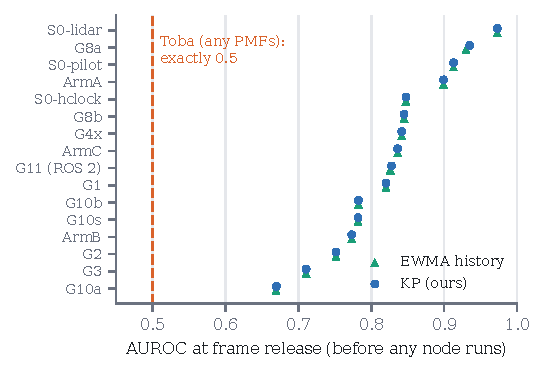
\includegraphics[width=0.62\textwidth]{figs/release_auroc.pdf}
\caption{Release AUROC for 16 cases across 57 hardware runs. Toba et al.'s score is constant at release (Theorem~\ref{thm:blind}); scores with cross-frame state can rank frames.}
\label{fig:release}
\end{figure}

\begin{figure}[t]
\centering
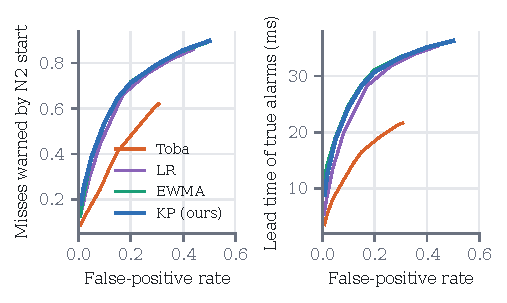
\includegraphics[width=0.62\textwidth]{figs/tradeoff.pdf}
\caption{Alarm trade-off with the same rule and a swept threshold for every method (mean of 57 runs). By the start of N2, history-based scores warn on about twice as many misses, and about twice as early, as plaxity.}
\label{fig:tradeoff}
\end{figure}

Figure~\ref{fig:release} confirms Theorem~\ref{thm:blind}. Across 57 runs on two platforms, with synthetic and LiDAR workloads in Python, C and ROS~2, plaxity's release AUROC was exactly 0.5. Scores based on history reached 0.64--0.97. The AUROC followed the Gaussian prediction in Proposition~\ref{prop:limit}, based on how much of the latency variation was explained by contention (Spearman correlation 0.56--0.74). This also explains the weaker cases: when contention explains little of the latency, no method has much to predict.

\begin{table}[t]
\caption{Open-loop comparison (means). A: 57 runs; B: Raspberry Pi~5, six fresh runs (visual odometry / LiDAR)}
\label{tab:open}
\footnotesize
\begin{tabular}{@{}lccc@{}}
\toprule
& Toba et al.~\cite{toba2026} & KP / KPF & LR \\
\midrule
\multicolumn{4}{@{}l}{\emph{A. At the thresholds recommended in~\cite{toba2026}}}\\
FPR & 0.89 & 0.51 & 0.44 \\
Precision & 0.29 & 0.40 & 0.43 \\
\multicolumn{4}{@{}l}{\emph{A. At FPR = 10\%}}\\
Misses warned by the start of N2 & 0.25 & 0.54 & 0.45 \\
Lead time of true alarms (ms) & 11.6 & 24.4 & 20.2 \\
\multicolumn{4}{@{}l}{\emph{B. KPF and LR on all features}}\\
Actionable AUROC & 0.67 / 0.81 & 0.89 / 0.96 & 0.89 / 0.96 \\
FPR needed for the long-run guarantee & 0.35 / 0.20 & 0.12 / 0.09 & -- \\
\bottomrule
\end{tabular}
\end{table}

At the thresholds recommended in~\cite{toba2026}, plaxity alarmed on 89\% of frames that met their deadlines. KP cut this rate by about half and performed better in 53 of 57 runs (Table~\ref{tab:open}). When we swept one threshold for all methods (Fig.~\ref{fig:tradeoff}), precision was nearly the same. By the start of N2, however, KP warned on 2.2 times as many misses and gave 2.1 times as much lead time. KP's actionable AUROC was higher than plaxity's in 52 of 54 earlier runs and all three pre-registered ROS~2 runs (by 0.14--0.27, with a block-bootstrap confidence interval above zero). Theorem~\ref{thm:aci} held in all 1{,}140 checked cases. By contrast, a threshold fixed using calibration data drifted to 2--4 times its target under unseen contention. In 106 of 114 cases, KP needed 1.5--3 times fewer false alarms than plaxity to meet the same long-run guarantee.

These results do not show that our predictor is better. Logistic regression with the same features ranked frames as well as or slightly better than KPF (actionable AUROC 0.893 versus 0.888 on the UNO~Q). The pre-registered test that KPF would rank better failed on both boards (2/6 and 3/6). A moving average of past latency captured most of the improvement over plaxity. KPF's remaining advantages were better calibration under unseen contention (expected calibration error 0.072 versus 0.128 for LR) and lower cost. In the Pi~5 open-loop test, rule \Wu{} met $(4,20)$ exactly: the worst window was 4.0, compared with 18.5 without a monitor and 7.3 with only the burst guard. It added 0.012 to the FPR. The same rule also held with LR and plaxity scores (36/36).

\subsection{Closed-Loop Evaluation: Latch-Up and Its Fix}\label{sec:eval-latch}

\begin{table}[t]
\caption{Closed loop on the Raspberry Pi~5 with the live ROS~2 LiDAR DAG, mean of three seeds (about 2{,}600 frames per policy). Last
column: worst number of unwarned misses in any 20 frames (for no action, misses that the passive monitor did not flag).}
\label{tab:latch}
\footnotesize
\begin{tabular}{@{}lcccc@{}}
\toprule
Policy & Missed & Degraded & Degraded in quiet periods & Worst unwarned per 20 \\
\midrule
No action & 36.7\% & 0\% & 0\% & 8 \\
Original monitor (\pol{kp}) & 9.4\% & 61.6\% & 30.0\% & 15.3 \\
Fixed monitor (\pol{kpm}) & 9.9\% & 43.8\% & \textbf{0.1\%} & 8 \\
Fixed monitor + \Wu{} (\pol{kpmwh}) & \textbf{8.7\%} & 43.1\% & 0\% & \textbf{4} \\
Toba et al.~\cite{toba2026} & 15.4\% & 48.4\% & 33.4\% & 10.7 \\
Random, same budget & 21.6\% & 43.5\% & 43.5\% & 16.7 \\
\bottomrule
\end{tabular}
\end{table}

Table~\ref{tab:latch} reports the pre-registered closed-loop Pi~5 test; eight of nine rules passed. At the same miss rate, the mode-aware update cut degradation during quiet periods from 30\% to 0.1\%. Rule \Wu{} held for every seed. Two findings limit this result. Our method did not degrade fewer frames than plaxity in two of the three seeds. Also, level-1 frames were still late 10--16\% of the time. Keeping half the point cloud is a lighter mode, but it is not a guaranteed fallback. A later UNO~Q test isolated the state update from the burst guard. The update alone degraded 0--0.7\% of quiet frames, compared with 63--100\% for the original monitor. The pre-registered ratio test for ``no latch'' still failed in two of three seeds because its reference rate was exactly zero. We count it as a failure.

\subsection{Closed-Loop Evaluation: All Late Frames}\label{sec:eval-all}

\begin{figure}[t]
\centering
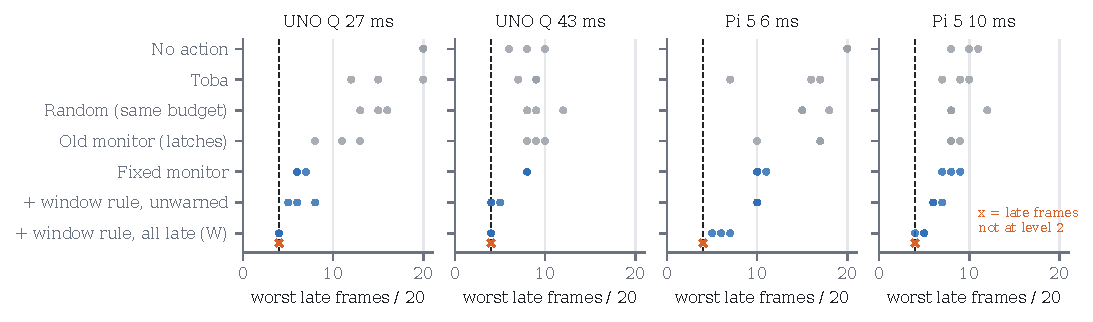
\includegraphics[width=\textwidth]{figs/closed_loop_windows.pdf}
\caption{Worst count of late frames in any 20-frame window for each seed in the live ROS~2 tests. The dashed line marks $m=4$. Crosses show late frames not run at level~2; Theorem~\ref{thm:all} limits this count to four without a timing assumption. UNO~Q: 27 and 43\,ms. Pi~5: 6 and 10\,ms. Each policy, seed and deadline has 2{,}000 scheduled releases; after removing contention-change releases and warm-up, about 1{,}700--1{,}800 frames remain.}
\label{fig:windows}
\end{figure}

Two pre-registered experiments tested all eight policies on new seeds at two deadlines per board (Fig.~\ref{fig:windows}). \emph{Theorem~\ref{thm:all} held in all 12 runs}: every 20-frame window had at most four late frames that were not at level~2. On the UNO~Q, all 790 level-2 frames finished on time. The plain bound therefore held in all six runs, with no more than four late frames per window, even under contention not seen during calibration. At 27\,ms, the other policies had worst windows of 5--20 late frames.

\emph{At 6\,ms on the Pi~5, the plain form failed.} Level~2 was late in 77 of 1{,}312 frames (5.9\%). The worst windows contained 7, 5 and 6 late frames, so the pre-registered plain-form test failed in all three seeds. This result challenges assumption A, not the rule: every late frame beyond four was a late level-2 frame, as Theorem~\ref{thm:all} allows. The worst windows of late level-2 frames contained 5, 1 and 5. Rule \Wl{} still had the smallest worst window in each seed (the other policies had 7--20, with one tie). Its mean miss rate across the three seeds was 9.3\%, compared with 15.0\% for plaxity and 22.1\% for random degradation. These averages are descriptive; they do not show that our policy had the lowest miss rate in every seed and were not a pre-registered claim. At 10\,ms, only two late level-2 frames among 243 were enough to break the plain bound by one in two of the three runs. A hard bound can fail even when fallback misses are rare.

\subsection{Replication on Seven New Seeds}\label{sec:eval-repl}

We repeated the UNO~Q closed-loop test on seven new seeds (261--267) to see whether the earlier results depended on the original three seeds. The addendum (Addendum S) was frozen before collecting any new data. It used the same eleven rules, code and calibration procedure as the original experiment. We recorded md5 checksums for the rules, analysis script and board scripts when we froze the plan. A reboot during seed 264 erased an unflushed calibration file. We reran that seed's calibration from the start and kept the lost files. The only change to the phase script was to flush files to disk. Calibration set the heavy deadline to 27\,ms on six seeds and 26\,ms on one. Light deadlines were 42--44\,ms. Each of the 112 runs had 2{,}000 scheduled releases, of which about 1{,}700--1{,}800 remained after the same filtering.

\emph{All guarantee tests passed.} Level-2 frames were on time in all 14 runs: none of the 1{,}754 frames was late. The exact form of Theorem~\ref{thm:all} held in all 14 runs, and so did the plain form. In every \pol{kpmd} run, the worst window contained exactly four late frames; at the heavy deadline, the worst windows for \pol{none}, \pol{toba} and \pol{random} contained 11--20. The long-run bound held in all 42 checks. The inline cost stayed below 200\,\textmu s at the 99th percentile in all 14 runs. Across all ten UNO~Q seeds, Theorem~\ref{thm:all} and Corollary~\ref{cor:A} held in all 20 runs. None of the 2{,}544 level-2 frames was late (95\% upper bound: 0.12\%).

\emph{Five comparison rules failed and remain failed.} Under the ratio rule, the isolated update \pol{kpmn} avoided latch-up in only 3 of 7 seeds (P5 required 7 of 7). At the light deadline, \pol{kpm} missed fewer frames than no monitor in 4 of 7 seeds (P7a required 7 of 7) and no more than random degradation in 4 of 7 (P7b required 6 of 7). Across the ten seeds, its mean miss rate was 5.2\%, compared with 5.8\% without a monitor and 5.4\% with random degradation. So the monitor did not reliably reduce misses at light load. The spread in degraded fractions was 0.31 for \pol{kpm} and 0.58 for plaxity, not less than half as required by P8. The fallback policy \pol{kpmd} had no more late frames than \pol{kpmwh} in only 7 of 14 runs (P11 required 12 of 14). The policies tied on total late frames; the fallback adds a window bound on all late frames, not fewer late frames. At the heavy deadline, every policy with the guarantee layer had a mean miss rate of 4.2--4.8\% across the ten seeds, compared with 33.3\% without a monitor, 16.4\% with random degradation and 18.0\% with plaxity. These are descriptive averages, not a pre-registered rule. The replication supports the guarantees but does not support the comparative advantages at light load.

\subsection{Validation of the Fallback Assumption}\label{sec:eval-fb}

\begin{figure}[t]
\centering
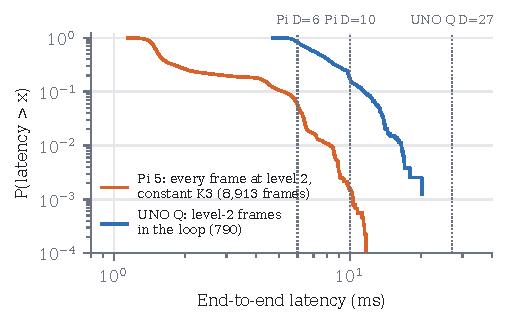
\includegraphics[width=0.62\textwidth]{figs/fallback_ccdf.pdf}
\caption{Latency distribution for level-2 frames. On the Pi~5, each frame ran at level~2 under constant contention from three interferers (three seeds). The UNO~Q data are level-2 frames from the closed-loop tests. Pi~5 median latency was 1.5\,ms, but the tail reached 12\,ms.}
\label{fig:fallback}
\end{figure}

We tested assumption A on the Pi~5 by running every scheduled frame at level~2 while three interferers created constant contention (Fig.~\ref{fig:fallback}). The confirmatory arm scheduled 3{,}000 releases for each of three seeds (a separate 1{,}000-release arm at another contention level was exploratory and is not used here). We excluded the nine releases per seed that overlapped the start-up contention change and the first 20 remaining releases as warm-up, leaving 8{,}913 frames. As the pilot suggested, level~2 missed the 6\,ms deadline: 2.3--10.2\% of retained frames were late in each seed. At 10\,ms, 13 of 8{,}913 frames were late (0.15\%; 95\% Clopper--Pearson~\cite{clopper1934} upper bound: 0.23\%). The long tail was not due to the amount of work. Median latency was 1.5\,ms, divisors from 2 to 32 behaved similarly in the pilot, and pinning interferers to other cores did not remove the tail. The cause was operating-system scheduling under contention.

We pre-registered a follow-up test of whether running the background load under \texttt{SCHED\_IDLE}, without root privileges, would make level~2 meet the 6\,ms deadline. The board became unreachable during the confirmatory runs, and we could not retrieve the data. We do not report or use a result from that test.

Table~\ref{tab:ledger} lists each guarantee, its premise and the evidence for that premise on each setup. On the UNO~Q, none of the 2{,}544 level-2 frames in ten closed-loop seeds was late; the 95\% upper bound on the per-frame late rate is 0.12\%. A pre-registered stress test (Addendum S, rule S12: no more than 0.5\% late at 27\,ms) ran every frame at level~2 under heavy contention, with 4{,}000 releases for each of three seeds. Using the same filter as the Pi~5 test (1--5 contention-change releases and 20 warm-up releases removed per seed), 4 of 11{,}929 frames were late at 27\,ms (0.034\%; 95\% upper bound: 0.077\%; the rule passed). At most three were late in any 20-frame window. Two were late at 43\,ms. Median latency was 7.6--8.0\,ms, and the worst was 80\,ms. These results support A on the UNO~Q, but do not prove it: the fallback was rarely late. A system designer should use Corollary~\ref{cor:r} with a small $r$ rather than rely on Corollary~\ref{cor:A}. At 10\,ms on the Pi~5, the late rate was low but not zero, so only Theorem~\ref{thm:all} and Corollary~\ref{cor:r} apply. At 6\,ms, assumption A was false. The $r$ values in Table~\ref{tab:ledger} come from these same runs and describe only those runs; a deployed design would need to set $r$ using separate qualification tests. Late level-2 frames can cluster (up to five in one window at a 5.9\% rate), so designers must measure $r$ per window rather than infer it from the average rate using an independence assumption. The guarantees on \emph{unwarned} misses do not depend on A. Theorem~\ref{thm:aci} held in all 36 policy runs across these two tests, and every \pol{kpmwh} and \pol{kpmd} run on both boards had a worst unwarned-miss window of exactly four.

\begin{table}[t]
\caption{Which window guarantee on late frames holds where (rule \Wl, $(m,K)=(4,20)$; UNO~Q: ten seeds at two deadlines, Pi~5: three seeds per deadline). ``Held'' and
``failed'' are observed outcomes; the premise is what a claim requires.}
\label{tab:ledger}
\footnotesize
\begin{tabular}{@{}p{0.27\textwidth}p{0.2\textwidth}ccc@{}}
\toprule
Guarantee & Premise & \makecell{UNO~Q\\27, 43\,ms} & \makecell{Pi~5\\10\,ms} & \makecell{Pi~5\\6\,ms} \\
\midrule
Theorem~\ref{thm:all}: late frames not at level 2 $\le m$ & none & held 20/20 & held 3/3 & held 3/3 \\
Corollary~\ref{cor:r}: late frames $\le m+r$ & at most $r$ late level-2 frames per window & $r=0$ & $r=1$ & $r=5$ \\
Corollary~\ref{cor:A}: late frames $\le m$ & A: level 2 never late & held 20/20 & \textbf{failed} 2/3 & \textbf{failed} 3/3 \\
\midrule
\multicolumn{2}{@{}l}{Late level-2 frames, closed loop} & 0 of 2{,}544 & 2 of 243 & 77 of 1{,}312 \\
\multicolumn{2}{@{}l}{Level-2 late rate, 95\% upper bound} & 0.12\% & 2.6\% & 7.1\% \\
\multicolumn{2}{@{}l}{Level-2 late, constant stress} & 0.034\% (27\,ms) & 0.15\% & 2.3--10.2\% \\
\multicolumn{2}{@{}l}{Status of assumption A} & supported (rare late) & false (rare) & false \\
\bottomrule
\end{tabular}
\end{table}

\subsection{Verification of the Theorems and the Implementation}\label{sec:eval-verify}

The proofs in Section~\ref{sec:method} are short. We also need to check that the deployed code follows the rules in those proofs. We used three independent checks.

\paragraph{Exhaustive state-space search} The first checker explores every reachable abstract state for rules \Wu{} and \Wl{}. It covers 38{,}900 states for $K\le7$, $m<K$ and lags up to 2, plus selected cases up to $K=10$. It also catches both negative controls: a counter that ignores running frames, and a level~2 fallback that can be late.

\paragraph{Independent exhaustive enumeration} We wrote a second checker from scratch in C, without sharing code with the first. It enumerates all predictor decisions, outcomes and completion delays up to horizon $T$, simulates the rules and checks every window. It covers $K\le5$, $m<K$, $L\le3$, and $T$ from 8 to 14. Across about 5.4 billion sequences, it found no violation of Theorems~\ref{thm:wu} and~\ref{thm:all} or Proposition~\ref{prop:min}. It also confirmed that a counter which counts only known outcomes can allow exactly $\min(m+L-1,K)$ unwarned misses per window (Proposition~\ref{prop:need}(3)); the lag effect is therefore tight. The checker caught an off-by-one version of rule \Wu{} used as a negative control. Using integer arithmetic, it also checked every alarm and outcome sequence permitted by the threshold for $T\le14$, $L\le2$ and three initial thresholds. It found no violation of Theorem~\ref{thm:aci}. A third enumeration checked Theorem~\ref{thm:cost} for all $K\le6$, $m<K$ and $L\le3$, across about 15 billion sequences. It found no violation and, for $L=1$, confirmed that the maximum $mF/U$ is exactly $K-m$.

\paragraph{Implementation conformance} We replayed the closed-loop logs from Section~\ref{sec:eval-all}. For every release in every \pol{kpmd} and \pol{kpmwh} run on both boards, we recalculated the counter from the logged completion times using the rule's definition. We then compared the resulting decision with the deployed C++ implementation. All 48{,}000 decisions matched, including UNO~Q frames that took up to 289\,ms and stayed active across several releases. The logs also satisfy Theorem~\ref{thm:cost} in all 12 \pol{kpmwh} runs. Rule \Wu{} forced 2.3--12.5\% of frames. The worst-case bound, $(K-1)U/m$, was 2.6--7.7 times higher because real misses did not occur in the worst-case adversarial pattern.

These checks are not formal proofs, and the exhaustive tests cover only small parameter values. They help catch mistakes in the arguments and code; the formal proofs remain the basis for our claims.

\subsection{Calculation Time and Downstream Value}\label{sec:eval-cost}

The inline monitor with rule \Wl{} takes 14--27\,$\mu$s per frame at the 99th percentile on the Pi~5 and 54--84\,$\mu$s on the UNO~Q, less than 0.1\% of either board's period. On the UNO~Q, plaxity takes 3.6\,$\mu$s at the median. We also simulated an unstable plant controlled by LQR, using state estimates from recorded Pi~5 traces. With KPF and the guarantees, its control cost was 5--10 times lower than with no monitor. It had no crashes and lower cost than with plaxity's score; all five pre-registered rules passed. For this simulated plant, the certificate in Section~\ref{sec:all} gives a worst 20-frame block gain of 0.001--0.14 across eight plant settings and six budgets. Without a bound, holds make the state grow by 1.2--2.7 times per frame. The plant was simulated, but we measured the window bound required by the certificate on hardware.

\subsection{Discussion and Limitations}\label{sec:eval-disc}

\paragraph{Choosing the window contract} Choose $(m,K)$ based on how many consecutive or clustered late outputs the downstream controller can tolerate. The monitor enforces this contract, but it cannot tell whether a particular controller remains stable under it. Evaluate the certificate in Section~\ref{sec:all} for the intended plant and controller. Corollary~\ref{cor:cost} also shows the cost: the forced-frame fraction is at most $(K-1)\alpha/m$. Exploratory UNO~Q runs, which were not pre-registered, showed the expected trade-off. When the window budget was much tighter than the long-run unwarned-miss rate, the rule warned on frames the predictor considered safe.

\paragraph{Qualifying the fallback} Theorem~\ref{thm:all} does not assume the fallback meets its deadline. Claim the plain $(m,K)$ bound only when level~2 is known to finish on time, for example through a WCET argument or a reservation. If level-2 misses still occur, independently establish a per-window limit $r$ and use Corollary~\ref{cor:r}. An average miss rate is not enough because late level-2 frames can cluster.

\paragraph{Choosing the predictor} Because the guarantees do not depend on the score, choose a predictor based on false-alarm cost, how well it stays calibrated under unseen contention, its implementation cost and the available telemetry. A moving average of past latency captured most of the improvement over per-frame plaxity. Logistic regression ranked frames as well as or slightly better than KPF. Our results support using information from earlier frames; they do not show that the Kalman predictor is the best model.

\paragraph{Scope and threats to validity} Our closed-loop tests use one main LiDAR DAG on two boards. Different seeds on one board do not count as separate hardware platforms. We tested visual odometry only in the open-loop replication. We reimplemented Toba's method from its published equations because the original implementation was unavailable. We have no WCET proof for level~2. The downstream control test uses hardware traces but simulates the plant. We did not use real-time priorities, CPU isolation or memory-bandwidth reservations, so we do not know how those mechanisms would affect the fallback's long-latency tail.

\subsection{Summary of Claims, Premises and Status}\label{sec:eval-claims}

Table~\ref{tab:claims} lists each claim, its premise and its status, including failed claims.

\begin{table}[t]
\caption{Claims, premises and status. ``Pre-registered'' gives the frozen rules passed out of the total.}
\label{tab:claims}
\footnotesize
\begin{tabular}{@{}p{0.43\textwidth}p{0.24\textwidth}p{0.25\textwidth}@{}}
\toprule
Claim & Premise & Status \\
\midrule
Plaxity cannot rank frames at release (Theorem~\ref{thm:blind}) & none & proven; observed in 57/57 runs \\
Cross-frame state ranks frames at release & contention present & AUROC 0.64--0.97 \\
The predictor outranks logistic regression & -- & \textbf{failed} (2/6, 3/6) \\
Long-run bound on unwarned misses (Theorem~\ref{thm:aci}) & none & proven; held in every run \\
$(m,K)$ on unwarned misses, minimal (Theorem~\ref{thm:wu}, Prop.~\ref{prop:min}) & none & proven; held in every run \\
All late frames, exact form (Theorem~\ref{thm:all}) & bookkeeping (verified) & proven; held 26/26 \\
All late frames, plain form (Corollary~\ref{cor:A}) & fallback never late & held 20/20 on UNO~Q; \textbf{failed} on Pi~5 (held in 0/3 runs at 6\,ms and 1/3 at 10\,ms) \\
Fallback rarely late on the UNO~Q under stress & -- & 0.034\% late (S12 passed) \\
Replication on 7 new seeds, guarantee rules & -- & passed (P1--P3, P9, P10) \\
Replication, comparative rules & -- & \textbf{failed} (P5, P7a, P7b, P8, P11) \\
Fallback on time at 6\,ms on the Pi~5 & -- & \textbf{false} (pre-registered prediction) \\
Latch-up is fixed by the mode-aware update & -- & quiet-period degradation 30\% $\to$ 0.1\% \\
Fewer degraded frames than plaxity & -- & \textbf{failed} (1/3, twice) \\
Stability in the loop & window bound + plant & simulated plant only \\
\bottomrule
\end{tabular}
\end{table}

% =====================================================================================================================================
\section{Related Work}\label{sec:related}

Table~\ref{tab:compare} summarizes the related work discussed here.

Yano and Azumi~\cite{yano2023access} introduced early detection for DAG deadline misses. They derive each job's time limit from the end-to-end deadline and WCETs in a DAG with timer-driven and event-driven nodes. Toba and Azumi~\cite{toba2024} replaced WCETs with probabilistic execution times, and Toba, Baruah and Azumi~\cite{toba2026} added probability thresholds that depend on the remaining workload. These methods score each job from its elapsed time and assume independent execution times. We build on their score by adding cross-frame state and a guarantee layer. Pythia-MCS~\cite{jiang2020pythia} predicts overruns from I/O behavior and triggers mixed-criticality mode changes, but does not give a window guarantee.

Probabilistic timing analysis combines execution-time distributions to bound response times~\cite{bernat2002pwcet,davis2019survey}. Markov and hidden-Markov execution-time models~\cite{frias2017,friebe2023}, along with correlation-tolerant analyses~\cite{markovic2023cta,markovic2024caa}, estimate deadline-miss probabilities offline when execution times are dependent. These methods answer a design-time question. Our method makes online decisions and uses contention as a source of information. ROS~2 response-time analysis is available for reservation-based scheduling~\cite{casini2019ros2}, which we did not use. Memory-bandwidth controls~\cite{yun2013memguard} can reduce the contention our predictor uses and may also help the fallback meet its deadline.

Bernat, Burns and Llamos\'i~\cite{bernat2001weakly} formalized weakly-hard constraints. Section~\ref{sec:position} compares bounded-miss scheduling~\cite{bernat2001bms,hamdaoui1995} and weakly-hard monitoring~\cite{peeck2021,wu2020rv} with our method. In control, deadline-miss-aware methods~\cite{pazzaglia2019dmac} and stability analyses for weakly-hard miss patterns~\cite{maggio2020,vreman2021} design or check controllers for specified patterns. Our method produces such a pattern on hardware and measures the assumption it requires. The fallback follows the Simplex architecture~\cite{sha2001simplex}.

Our long-run bound is the one-sided form of adaptive conformal inference~\cite{gibbs2021}. Prior work has studied how validity changes when a model's output affects its future inputs~\cite{fannjiang2022}. Intervention latch-up is a concrete example of this feedback problem in a timing monitor.

% =====================================================================================================================================
\section{Conclusion}\label{sec:concl}

We presented a deadline-miss early-warning method for DAG tasks that keeps its guarantees when the system acts on warnings. Per-frame plaxity cannot rank frames at release, but a state carried across frames can use contention information to do so. Above either score, a guarantee layer limits the long-run rate of unwarned misses and, with lag-aware counting, the number of unwarned misses in every window while forcing as few warnings as possible. With a lighter fallback, it also gives an exact bound on all late frames and shows how that bound changes when the fallback is late. We identified and fixed intervention latch-up. Pre-registered tests on two embedded boards, an exhaustive theorem check and a replay of the deployed implementation confirmed the theorems. The plain bound held only where the fallback met its deadline: it held on the UNO~Q, including a replication on seven new seeds, but failed on the Pi~5 at 6\,ms. In that setting, the exact form is the guarantee to use. The replication did not confirm all comparison claims: at light load, the monitor did not reliably reduce misses, and the fallback did not reduce the total number of late frames.

Future work should establish, rather than only measure, that the fallback meets its deadline. We plan to test it with a reservation~\cite{casini2019ros2} or memory-bandwidth control~\cite{yun2013memguard} on a platform that supports those mechanisms, and to set the budget $r$ in Corollary~\ref{cor:r} using qualification tests. We also plan to test multi-rate DAGs with timer-driven and event-driven nodes~\cite{yano2023access,toba2026}, and to move from a simulated plant to a physical control loop.

\begin{acks}
Acknowledgments are omitted from this version.
\end{acks}

\bibliographystyle{ACM-Reference-Format}
\bibliography{refs}

\end{document}
